%% LyX 1.2 created this file.  For more info, see http://www.lyx.org/.
%% Do not edit unless you really know what you are doing.
\documentclass[oneside,english]{amsart}
\usepackage[T1]{fontenc}
\usepackage[latin1]{inputenc}
\usepackage{graphicx}

\makeatletter

%%%%%%%%%%%%%%%%%%%%%%%%%%%%%% LyX specific LaTeX commands.
\providecommand{\LyX}{L\kern-.1667em\lower.25em\hbox{Y}\kern-.125emX\@}

%%%%%%%%%%%%%%%%%%%%%%%%%%%%%% Textclass specific LaTeX commands.
 \theoremstyle{plain}    
 \newtheorem{thm}{Theorem}[section]
 \numberwithin{equation}{section} %% Comment out for sequentially-numbered
 \numberwithin{figure}{section} %% Comment out for sequentially-numbered
 \theoremstyle{definition}
  \newtheorem*{example*}{Example}

%%%%%%%%%%%%%%%%%%%%%%%%%%%%%% User specified LaTeX commands.
\usepackage{epic,eepic,epsfig}
\newcommand{\define}{\stackrel{\mathrm{def}}{=}

\usepackage{babel}
\makeatother
\begin{document}

\title{Lectures 9\&10 ----Other Markov Queues}


\author{Neil Lawrence}

\maketitle

\subsection*{Statistical Multiplexing vs Time and Frequency division}

Example 3.9 in Bertsekas \& Gallager

Assume we have m statistically independent Poisson streams. Each has
arrival rate $\frac{\lambda }{m}$. Each has an average transmission
time $\bar{X}$. 

If we merge the Poisson streams together, through statisical multiplexing,
property of Poisson from Lecture 3\&4 tell us that they become a Poisson
stream with rate $\lambda $. Average delay, from last lecture will
be\[
\bar{T}=\frac{1}{\mu -\lambda }.\]
Now consider an alternative approach of providing each channel with
a seperate circuit. This involves splitting our transmission line
into $m$ channels. Each will now have bandwidth at most $\frac{\mu }{m}$.

Delay in this system will now be\[
\bar{T}=\frac{1}{\frac{\mu }{m}-\frac{\lambda }{m}}=\frac{m}{\mu -\lambda }\]
or $m$ times larger than statistical multiplexing. 

Why does this happen?

Consider the situtation where there is only one packet in the system.
In this case much of the bandwidth will be redundant.


\subsection*{Kendall's notation}

Arrival Charateristics/Departure Charateristics/number of servers/maximum
number of customers


\subsubsection*{Arrival and Departure Charateristics}

\begin{itemize}
\item $M$- Markov - Poisson distributed arrivals, exponentially distributed
service times.
\item $D$ - Deterministicly distributed times.
\item $G$ - General distribution for inter-arrival/service times.
\end{itemize}

\subsection*{Finite Length $M$/$M$/$1$/$m$}

So far we have assumed that the queue can have an infinite length.
What if it has a restricted buffer of size $m$? 

Insert diagram here

Let us assume the queue can contain at maximum $m$ arrivals. The
balance equation from above still applies. However, now the normalisation
is different, giving a different value for $P(0)$. \[
\sum _{k=0}^{m}P(0)\rho ^{k}=1\]
 Since this is simply a finite sum of a geometric series \[
P(0)=\frac{1}{\sum _{k=0}^{m}\rho ^{k}}=\frac{1-\rho }{1-\rho ^{m+1}}\]
 We therefore have \[
P(k)=\frac{\rho ^{k}(1-\rho )}{1-\rho ^{m+1}}\]


Given a finite length $M$/$M$/$1$/$m$ queue, what is the probability
that an arrival is blocked from joining the queue (and therefore lost). 

This is answered by determining the probability of the queue being
full, which means \[
P(m)=\frac{\rho ^{m}(1-\rho )}{1-\rho ^{m+1}}\]



\section*{$M$/$M$/$\infty $}

Insert diagram here


\subsection*{Detailed Balance }

\begin{eqnarray*}
\lambda _{k-1}P\left(k-1\right) & = & \mu _{k}P\left(k\right)\\
\lambda P\left(k-1\right) & = & k\mu P\left(k\right)
\end{eqnarray*}
thus we can write\[
P\left(k\right)=\frac{\lambda }{k\mu }P\left(k-1\right)\]
and therefore\[
P\left(k\right)=P\left(0\right)\left(\frac{\lambda }{\mu }\right)^{k}\frac{1}{k!}\]
using the normalisation conditions we can see that\begin{eqnarray*}
\sum _{k=0}^{\infty }P\left(k\right) & = & 1\\
P\left(0\right) & = & \left[\sum _{k=0}^{\infty }\left(\frac{\lambda }{\mu }\right)^{k}\frac{1}{k!}\right]^{-1}
\end{eqnarray*}
Define offered load, $a=\frac{\lambda }{\mu }$, as arrival rate divided
by service rate. This is a dimensionless constant, but has international
units of Erlangs. \[
P\left(0\right)=\left[\sum _{k=0}^{\infty }\frac{a^{k}}{k!}\right]^{-1}\]
recalling that $\exp \left(x\right)=\sum _{n=0}^{\infty }\frac{x^{n}}{n!}$
we have\[
P\left(0\right)=\exp \left(-a\right)\]
and the steady state distribution\[
P\left(k\right)=\frac{a^{k}}{k!}\exp \left(-a\right)\]
which is recognised as a poisson distribution with parameter $a$.


\section*{Erlang Delay $M$/$M$/$m$}

The Erlang Delay system. In Kendall's notation Generally for circuit
switched networks 

Define average holding time, $\tau =\frac{1}{\mu }\equiv \bar{X}$,
time a call is open. {\small }%
\begin{figure}
\begin{center}\input{./diagrams/erlangDelayDiagram.eepic}\end{center}


\caption{Queueing model of the Erlang delay system.}
\end{figure}
{\small \par}

The Erlang loss system may be analysed as a birth-death process with
birth rate \[
\lambda _{k}=\lambda \]
 and death rate \[
\mu _{k}=\left\{ \begin{array}{cc}
 k\mu  & k=0,1,\dots ,m-1\\
 m\mu  & k>m\end{array}
\right.\]


{\tiny }%
\begin{figure}
\begin{center}\input{./diagrams/erlangDelay.eepic}\end{center}


\caption{State diagram of an Erlang delay system.}
\end{figure}
{\tiny \par}


\subsection*{Detailed Balance Equations}

For a system having state less than $m$, $k\leq m$ the detailed
balance equation is 

\[
\lambda P(k-1)=k\mu P(k)\]
therefore for $k=0\dots m$ we may write\[
P\left(k\right)=\frac{\lambda }{k\mu }P\left(k-1\right)\]
we define\[
\rho =\frac{\lambda }{m\mu }\]
and therefore\[
\frac{\lambda }{k\mu }=\frac{m\rho }{k}\]
therefore we may write\[
P\left(k\right)=\frac{m\rho }{k}P\left(k-1\right)\]
and as before\begin{eqnarray}
P\left(k\right)=\frac{\left(m\rho \right)^{k}}{k!}P\left(0\right) &  & \textrm{for }k\leq m\label{eq:probabilities}
\end{eqnarray}


For systems with state greater than $m$, $k>m$ the detailed balance
equation is\[
\lambda P(k-1)=m\mu P(k)\]
therefore for $k=m+1\dots \infty $ we may write\[
P\left(k\right)=\frac{\lambda }{m\mu }P\left(k-1\right)\]
and therefore\[
P\left(k\right)=\rho P\left(k-1\right)\]
leading to \[
P\left(k\right)=\rho ^{k-m}P\left(m\right)\]
and substituting $k$ with $m$ in (\ref{eq:probabilities}) we can
obtain\[
P\left(m\right)=\frac{\left(m\rho \right)^{m}}{m!}P\left(0\right)\]
therefore \begin{eqnarray*}
P\left(k\right)=\frac{m^{m}\rho ^{k}}{m!}P\left(0\right) &  & \textrm{for }k>m
\end{eqnarray*}
thus we can write\[
P(k)=\left\{ \begin{array}{cc}
 P(0)\frac{(m\rho )^{k}}{k!}, & k\leq m\\
 P(0)\frac{m^{m}\rho ^{k}}{m!} & k>m\end{array}
\right.\]


Once again we can compute $P\left(0\right)$ through normalisation\begin{eqnarray*}
\sum _{k=0}^{\infty }P\left(k\right) & = & 1\\
P\left(0\right)\left[\sum _{k=0}^{m-1}\frac{\left(m\rho \right)^{k}}{k!}+\sum _{k=m}^{\infty }\frac{m^{m}\rho ^{k}}{m!}\right] & = & 1\\
P\left(0\right) & = & \left[\sum _{k=0}^{m-1}\frac{\left(m\rho \right)^{k}}{k!}+\sum _{k=m}^{\infty }\frac{m^{m}\rho ^{k}}{m!}\right]^{-1}
\end{eqnarray*}


consider the second term inside the bracket\[
\sum _{k=m}^{\infty }\frac{m^{m}}{m!}\rho ^{k}=\frac{m^{m}\rho ^{m}}{m!}\sum _{k=m}^{\infty }\rho ^{k-m}\]


substitute in $k^{\prime }=k-m$ and we obtain\[
\frac{m^{m}\rho ^{m}}{m!}\sum _{k^{\prime }=0}^{\infty }\rho ^{k^{\prime }}=\frac{m^{m}\rho ^{m}}{m!}\frac{1}{1-\rho }\]


if $\rho <1$. Thus we have\[
P\left(0\right)=\left[\sum _{k=0}^{m-1}\frac{\left(m\rho \right)^{k}}{k!}+\frac{m^{m}\rho ^{m}}{m!\left(1-\rho \right)}\right]^{-1}\]
one quantity of interest is the probability of queueing, $P_{Q}$.
What is the probability, when the system is at steady state, that
a customer will arrive and find all the $m$ servers busy? \[
P\left(k\geq m\right)=\sum _{k=m}^{\infty }P\left(k\right)=P\left(0\right)\sum _{k=m}^{\infty }\frac{m^{m}\rho ^{k}}{m!}=P\left(0\right)\frac{\left(\rho m\right)^{m}}{m!}\sum _{k=m}^{\infty }\rho ^{k-m}\define P_{Q}\]
hmaking the same substitution as above this can be re-written\[
P_{Q}=\frac{P\left(0\right)\left(\m \rho \right)^{m}}{m!\left(1-\rho \right)}\define C\left(m,a\right)\]


This is known as the \emph{Erlang C formula}, or Erlang's second formula
after A.K. Erlang a pioneer of queueing theory. By defining, $a$,
the offered load to be\[
a=\frac{\lambda }{\mu }=m\rho \]
 and substituting into the above we have \[
C(m,a)=\frac{P(0)a^{m}}{m!\left(1-\frac{a}{m}\right)}.\]
Nowadays we can compute the probability of waiting on a computer,
however for the purposes of exams and exercises we will use the old
fashioned method of curves.\newcommand{\figureTextSize}{\tiny}

{\small }%
\begin{figure}
\begin{center}\input{./diagrams/erlangCCurves0to20.eepic}\end{center}


\caption{Erlang C curves.}
\end{figure}
{\small \par}

{\small }%
\begin{figure}
\begin{center}\input{./diagrams/erlangCCurves0to100.eepic}\end{center}


\caption{Erlang C curves.}
\end{figure}
{\small \par}

\begin{example*}
Consider the telephone trunking problem. A telephone exchange A is
to server 10,000 subscribers in a nearby exchange as shown in Figure
\ref{fig:exchange}. Suppose that during the busy hour, the subscribers
generate a Poisson traffic with a rate of 10 calls per minute, which
requires trunk lines to exchange B for an average holding time of
3 minutes per call. Determine the number of trunk lines needed for
a grade of service (probability of waiting) of 0.01.

Average call rate is $\lambda =10$ calls/minute. Average holding
time is $\tau =3$ minutes. Offered load $a=\lambda \tau $ is 30
Erlangs.

From the Erlang C curves it looks to be about 44.

%
\begin{figure}
\begin{center}\input{./diagrams/exchange.eepic}\end{center}


\caption{The telephone exchange.\label{fig:exchange}}
\end{figure}

\end{example*}
A customer service centre has an average holding time for calls of
8 minutes. In the busy hour, calls arrive at the centre at a rate
of one very two minutes. Inter-arrival times and service times are
exponentially distributed, how many personel are required to keep
the probability of waiting at 0.1.

From the plot 8.

The average number of calls in the Erlang Delay System \[
\bar{N}=\frac{\rho }{1-\rho }C(m,a)+m\rho \]
 These terms represent the average queue length and the average number
of busy lines. \[
\bar{N}_{Q}=\frac{\rho }{1-\rho }C(m,a)\]
 So the average waiting time is simply \[
\bar{W}=\frac{\bar{N}_{Q}}{\lambda }=\frac{C(m,a)}{m\mu (1-\rho )}\]


\begin{example*}
So what is the average waiting time for the telephone service centre
example? 
\end{example*}
$m=8$, $\mu =\frac{1}{8}$, $\rho =\frac{\lambda }{m\mu }=\frac{1}{2}$. 

delay is $\frac{0.1}{8\frac{1}{8}(1-\frac{1}{2})}=0.2$ minutes, or
12 seconds. 


\section*{Erlang Loss $M$/$M$/$m$/$m$}

%
\begin{figure}
\begin{center}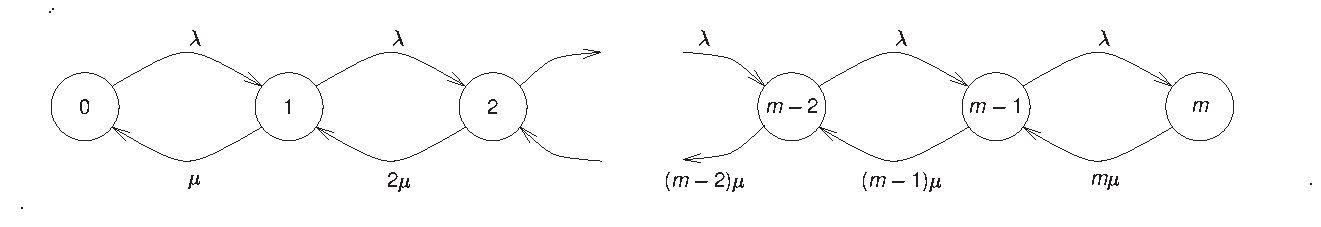
\includegraphics[  scale=0.5]{./diagrams/erlangLoss.eps}\end{center}


\caption{Flow chart of the Erlang Loss System.}
\end{figure}


The Erlang loss system may be analysed as a birth-death process with
birth rate \[
\lambda _{k}=\left\{ \begin{array}{cc}
 \lambda  & k=0,1,\dots ,m-1\\
 0 & k\geq m\end{array}
\right.\]
 and death rate \[
\mu _{k}=\left\{ \begin{array}{cc}
 k\mu  & k=0,1,\dots ,m\\
 0 & k>m\end{array}
\right.\]
 {[}\emph{Note: for the lower line, it doesn't matter what $\mu _{k}$
is.}{]} 

{\tiny }%
\begin{figure}
\begin{center}\input{./diagrams/erlangLoss.eepic}\end{center}


\caption{Markov chain for the Erlang loss system, $M$/$M$/$m$/$m$}
\end{figure}
{\tiny \par}

The offered load, $a=\frac{\lambda }{\mu }$, is again dimensionless
with units of Erlangs. 


\subsection*{Steady State Probabilities}

Using the global balance equations we find \begin{eqnarray*}
P(k) & = & \frac{\lambda _{k}}{\mu _{k}}P(k-1)\\
 & = & \frac{\lambda }{k\mu }P(k-1)\\
 & = & \frac{a}{k}P(k-1)
\end{eqnarray*}
 Which means that \begin{eqnarray*}
P(k) & = & \prod _{n=1}^{k}\frac{a}{n}P(0)\\
 & = & \frac{a^{k}}{k!}P(0)
\end{eqnarray*}
 The normalisation condition gives us \[
P(0)\sum _{k=0}^{m}\frac{a^{k}}{k!}=1\]
\[
P(0)=\frac{1}{\sum _{k=0}^{m}\frac{a^{k}}{k!}}\]
 which leads to the truncated Poisson distribution \[
P(k)=\frac{\frac{a^{k}}{k!}}{\sum _{n=0}^{m}\frac{a^{n}}{n!}}\]
 \textbf{Comment} This distribution also holds for $M$/$G$/$m$/$m$
queues --- not proven here. 

For the blocking probability and the Erlang B curves we are interested
in \[
B(m,a)=P(m)=\frac{\frac{a^{m}}{m!}}{\sum _{n=0}^{m}\frac{a^{n}}{n!}}\]
 {\small }%
\begin{figure}
\begin{center}\input{./diagrams/erlangBCurves0to20.eepic}\end{center}


\caption{Erlang B curves.}
\end{figure}
{\small \par}

{\small }%
\begin{figure}
\begin{center}\input{./diagrams/erlangBCurves0to100.eepic}\end{center}


\caption{Erlang B curves.}
\end{figure}
{\small \par}


\subsection*{Carried Load}

The carried load may be found as \[
a^{\prime }=a(1-P(m))=a(1-B(m,a))\]
 The carried load per line is the trunk occupancy, \[
\rho =\frac{a^{\prime }}{m},\]
 or the utilization factor --- it is a measure of efficiency. 

\begin{example*}
Load tripling.

For a blocking probability of 0.01, what is the number of trunks needed
for 6 erlangs of offered load? Answer 12

For a blocking probability of 0.01, what is the number of trunks needed
for 18 erlangs? Answer 30

So load increase of 200 \textbackslash{}\% only lead to a trunk increase
of 150 \textbackslash{}\%. Why? Let's look at the (approximate) utilization
factors. 

\begin{eqnarray*}
\rho _{1} & = & \frac{6}{12}\left(1-0.01\right)=0.495\\
\rho _{2} & = & \frac{18}{30}\left(1-0.01\right)=0.594
\end{eqnarray*}
 The 30 trunk system is thus more efficient.

This explains why it is cheaper to call the U.S.A. than Italy.
\end{example*}
\bibliography{/home/neil/tex/inputslawrence_books}

\end{document}
